%%%%%%%%%%%%%%%%%%%%%%%%%%%%%%%%%%%%%%%%%%%%%%%%%%%%%%%%%%%%%%%%%%%%%%%%
\chapter{Grundlagen}
\label{sec:fundamentals}
%%%%%%%%%%%%%%%%%%%%%%%%%%%%%%%%%%%%%%%%%%%%%%%%%%%%%%%%%%%%%%%%%%%%%%%%
\section{Software Qualitätssicherung}\todo[color=blue!40]{Feedback zu Struktur des Literaturkapitels}
\subsection{Motivation und Relevanz}

\todo{Evt. einleitende Worte...}
Der Funktionsumfang von Software stieg in den letzten fünzig Jahren enorm. Gleichzeitig bietet die Geschichte der Informatik viele Beispiele, die für die Notwendigkeit von Qualitätssicherung in der Softwareentwicklung sprechen. Ein sehr bildhaftes Beispiel der Folgen von fehlerhafter Software, ist die Selbstzerstörung der Ariane 5 Rakete im Jahr 1996 [QUELLE 1]\todo{Ref}. Das Trägheitsnavigationssystem wandelte eine 64-bit-Gleitkommazahl in eine Ganzzahl. Dieser Programmteil wurde schon in der Ariane 4 verwendet, nur war diese weitaus schubschwächer und der betroffene Sensor erzeugte viel kleinere Ergebnisse. Nur 36 Sekunden nach Start des Erstfluges, setzte also ein klassischer Überlauf ein und die Rakete aktivierte ihren Selbstzerstörungsmechanismus.
Ähnliches passierte bei der Raumsonde Mars Obiter der NASA. Diese war am 24. September 1999 gestartet und hätte 220 Millionen Kilometer später auf dem roten Planeten landen sollen. Kurz vor der Landung ging der Kontakt verloren, die Sonde zerschellte an der Oberfläche des Planeten. In diesem Fall war es kein Überlauf sondern ein Fehler bei den Maßeinheiten die den Steuerungsschub kontrollierten. Die Entwickler der NASA erwarteten in ihrem Code Zahlen in Form von Newton, während der Hersteller Lockheed Martin angloamerikanische Pfund lieferte.Durch Zufall fiel der Fehler während des gesamten Flugs nicht auf.[QUELLE 2 - 1]\todo{Ref} 
In keinem der beiden Vorfälle kamen Menschen zu Schaden, trotzdem waren die finanziellen Verluste enorm. Natürlich war die Komplexität dieser NASA-Projekte sehr hoch und wahrscheinlich nicht repräsentativ für Software die am Markt erhältlich ist, trotzdem wären beide Fehler durch Testing vermeidbar gewesen. Im Fall der Ariane 5 hätte es ausgereicht die Schnittstelle zum Steuercomputer mit Extremwerten zu testen. Man wäre schnell auf den Überlauf gestoßen und hätte die Umrechnung anpassen können. Auch Mars Orbiter hätte durch ausführliches Schnittstellen-Testing auf Basis von Verträgen, welche die beteiligten Software-Teams untereinander ausmachen, gerettet werden können.

\subsubsection{Der Zwang zu qualitativem Wachstum}
Die Qualität von Software erhöhte sich geschichtlich nicht im selben Maße wie ihre Funktionalität. Dafür werden von (Thaller)[QUELLE2 - 2]\todo{Ref} zwei Gründe genannt.

Der Drang nach Wachstum bei modernen Programmen negiert die Erfolge die Unternehmen durch erhöhte Anstrengungen in der Qualitätssicherung feiern könnten. Die Zahl der Fehler wird weitläufig gesenkt,  gleichzeitig nimmt der Funktionsumfang der Programme massiv zu. Dieser Umstand rührt daher, dass ständig neue Käuferschichten gewonnen werden müssen, die wiederum neue Features fordern.
Software dringt in Gebiete vor die von analoger Technik dominiert wurde. Aeronautik, Medizin und Finanzwesen verlangen nach großen Programmpaketen, die potenziell viele Fehlerquellen mit weichreichenden Folgen enthalten.

\subsubsection{Komplexe Systeme führen zu Fehlern}
Von der Programmierung in Hochsprachen bis zur Ausführung auf der Hardware müssen unzählige Schichten korrekt ineinander greifen um das gewünschte Ergebnis hervorzubringen. 
Daher sind

QUOTE „Komplexe Systeme analytisch in begrenzer Zeit nur unvollständig erfassbar. Fehler sind damit zwangsläufig die Folge“ [QUELLE3] \todo{Ref}

Gründe wieso Fehler auftreten sind mannigfaltig. Aus menschlicher Sicht können Fehler auf drei Ebenen auftreten [QUELLE 3]:\todo{Ref}

\paragraph{Kommunikation}
Jegliche Art von Kommunikation ist Transformation (vgl. SHANNON, 1976). Dabei passieren diese Transformationen nicht nur bei der Kommunikation zwischen zwei Menschen sondern auch bei der Transformation von Sprache in Verständnis. Naturgemäß bleibt bei diesen Transformationen Informationsgehalt verloren, abhängig von verschiedenen Rahmenbedingungen manchmal sogar sehr viel, beispielsweise wenn Information in einer Sprache übermittelt wird, welche nicht die Muttersprache von beiden Kommunikationspartnern ist.
Im technischen Umfeld gibt es darum viele Standardbegriffe, die möglichst genau definiert sind. So soll der Informationsverlust eingeschränkt werden.
Weiters spielt sich ein nicht unerheblicher Teil der Kommunikation auf unterbewusster Ebene ab.

\paragraph{Fachlichkeit}
Kunden oder Auftraggeber sind naturgemäß Experten auf ihrem Gebiet. Sie wollen Software um ihre fachlichen Ziele effektiver verfolgen zu können. Dem Software-Entwickler fehlt dieses Fachwissen. Dem Entwickler fehlt dieses Fachwissen oft.
Der Kunde hat sehr detaillierte Vorstellungen der Software, ihm fehlt aber die Fähigkeit auf technischer und fachlicher Ebene zu abstrahieren. Dies ist eine der Hauptaufgaben des Requirements-Engineer. Genau an dieser Stelle ist die Gefahr groß, dass durch fehlendes fachliches Wissen wichtige Zusammenhänge übersehen werden oder unwichtigen Details zu viel Aufmerksamkeit geschenkt wird.
Außerdem sind die technischen Möglichkeiten nur eingeschränkt für den Kunden fassbar. Gerade Aufwandsschätzungen sind für Entwickler schon schwierig Das hat zur Folge, dass die Entwickler oft Alternativen anbieten müssen welche möglicherweise nicht den exakten Anforderungen entsprechen.

\paragraph{Komplexität}
Die Komplexität der Problemstellung bestimmt über Machbarkeit und Fehlerpotenzial. Seit Anbeginn der Informatik wird versucht Komplexität auf ein überschaubares Maß herunterzubrechen. Sei es durch Zerlegung in möglichst kleine Aufgaben, visuelle Darstellungsformen oder Abstraktion zu bekannten Programmiermustern.
Komplexität wird dadurch aber niemals vermindert, sondern nur versteckt bzw. anschaulicher gemacht.


\subsection{Softwarequlität und Standards}
\subsection{Testprozess}
\subsection{Teststufen}
\subsubsection{Klassisches Vorgehen}
\subsubsection{Agiles Testen}
\subsection{Regressionstests und Testautomatisierung}
\subsection{Modellbasiertes Testen}
\subsubsection{Idee}
\subsubsection{Vergleich mit klassischem Testing}
\subsubsection{Tool-Landschaft}

\section{State of the Art - Modellbasiertes Testen}
In diesem Kapitel werden die theoretischen Grundlagen und alle in der Arbeit verwendeten und für das Verständnis relevante Begriffe erläutert. Kapitelnamen spezifizieren, anpassen an die Fragestellung der Arbeit.

\makeatletter\ifthesis@masterthesis
Nach dem Lesen dieses Kapitels sollten folgende Punkte klar dargestellt sein:
\begin{itemize}
	\item Beschreibung der relevanten theoretischen Grundlagen für die Behandlung der Fragestellung
	\item Detaillierte Beschreibung ggf. vorhandener relevanter Spezifika des Anwendungsbereichs, in dem das Problem gelöst wird
	\item Detaillierte Beschreibung relevanter Spezifika eingesetzter Technologien
	\item Analyse bestehender Ansätze/ Vorarbeiten: Literaturstudium, Analyse, Vergleich und Zusammenfassung bestehender Ansätze.
\end{itemize}
\fi\makeatother

Gerade im Bereich der Grundlagen wird viel Literatur zitiert -- Details zum Zitieren finden Sie im Kapitel \ref{sec:references}. Da keine Diplomarbeit so innovativ ist, dass sie nicht auf vorhandenes Wissen aufbaut und in ein entsprechendes Forschungsumfeld eingebettet ist, kommt an dieser Stelle der Literaturrecherche eine besondere Bedeutung zu. Als Daumenregel gilt, dass der aktuelle Stand der Wissenschaft in der Informatik üblicherweise durch Publikationen v.a. der letzten 2 – 4 Jahre repräsentiert wird.

\makeatletter\ifthesis@masterthesis
Beispielhaft einleitender Text an dieser Stelle:\\
Dieses Kapitel stellt Konzepte der Informationstheorie vor und liefert theoretische Grundlagen zu verdeckten Kanälen. Die verdeckte Kommunikation wird mit den verwandten Techniken der Steganographie und Kryptographie verglichen. Außerdem werden ein einfaches Fehlerkorrekturverfahren sowie die Grundlagen des HTTP-Protokolls beschrieben.
\fi\makeatother

State of the art
In diesem Kapitel wird ein Überblick über bereits existierende Lösungen für die Problemstellung bzw. verwandte Problemstellungen gegeben. Dabei ist eine Klassifizierung der existierenden Lösungen empfehlenswert. Eine Analyse der Lösungen, nach Kriterien sortiert, sollte insbesondere auch die Defizite der existierenden Lösungen erläutern und damit insbesondere auch eine Begründung liefern, warum diese Lösungen für die Problemstellung der Arbeit nicht herangezogen werden können.

Unterkapitel----------------------------------------------------------------------

Bei der Verwendung von Gliederungsebenen gibt es Folgendes zu beachten:
\begin{itemize}
	\item Es sollten nicht mehr als 3 Gliederungstiefen nummeriert werden.
	\item Unterkapitel sind nur dann sinnvoll, wenn es auch mehrere Untergliederungen gibt. Ein Kapitel 2.1.1 sollte somit nur dann verwendet werden, wenn es auch 2.1.2 gibt.
	\item Oft ist es einfacher und besser verständlich, Aufzählungen als Text zu formulieren und somit weitere Gliederungsstufen zu vermeiden.
\end{itemize}

Abbildungen
Beschreibungen zu Abbildungen und Tabellen stehen unter dem Bild. Jede Abbildung muss im Fließtext referenziert werden. In \LaTeX besitzen Abbildungen typischerweise Labels, welche zum referenzieren verwendet werden. Zudem plaziert \LaTeX die Abbildungen an geeigneten Stellen, was meistens auch wünschenswert ist. Falls das nicht gewünscht wird, kann es durch Optionen beeinflusst werden.

Abbildung \ref{fig:xxx} verdeutlicht  \dots\\
(siehe Abbildung \verb|\ref{<label>}|)

\begin{figure}
	\centering
	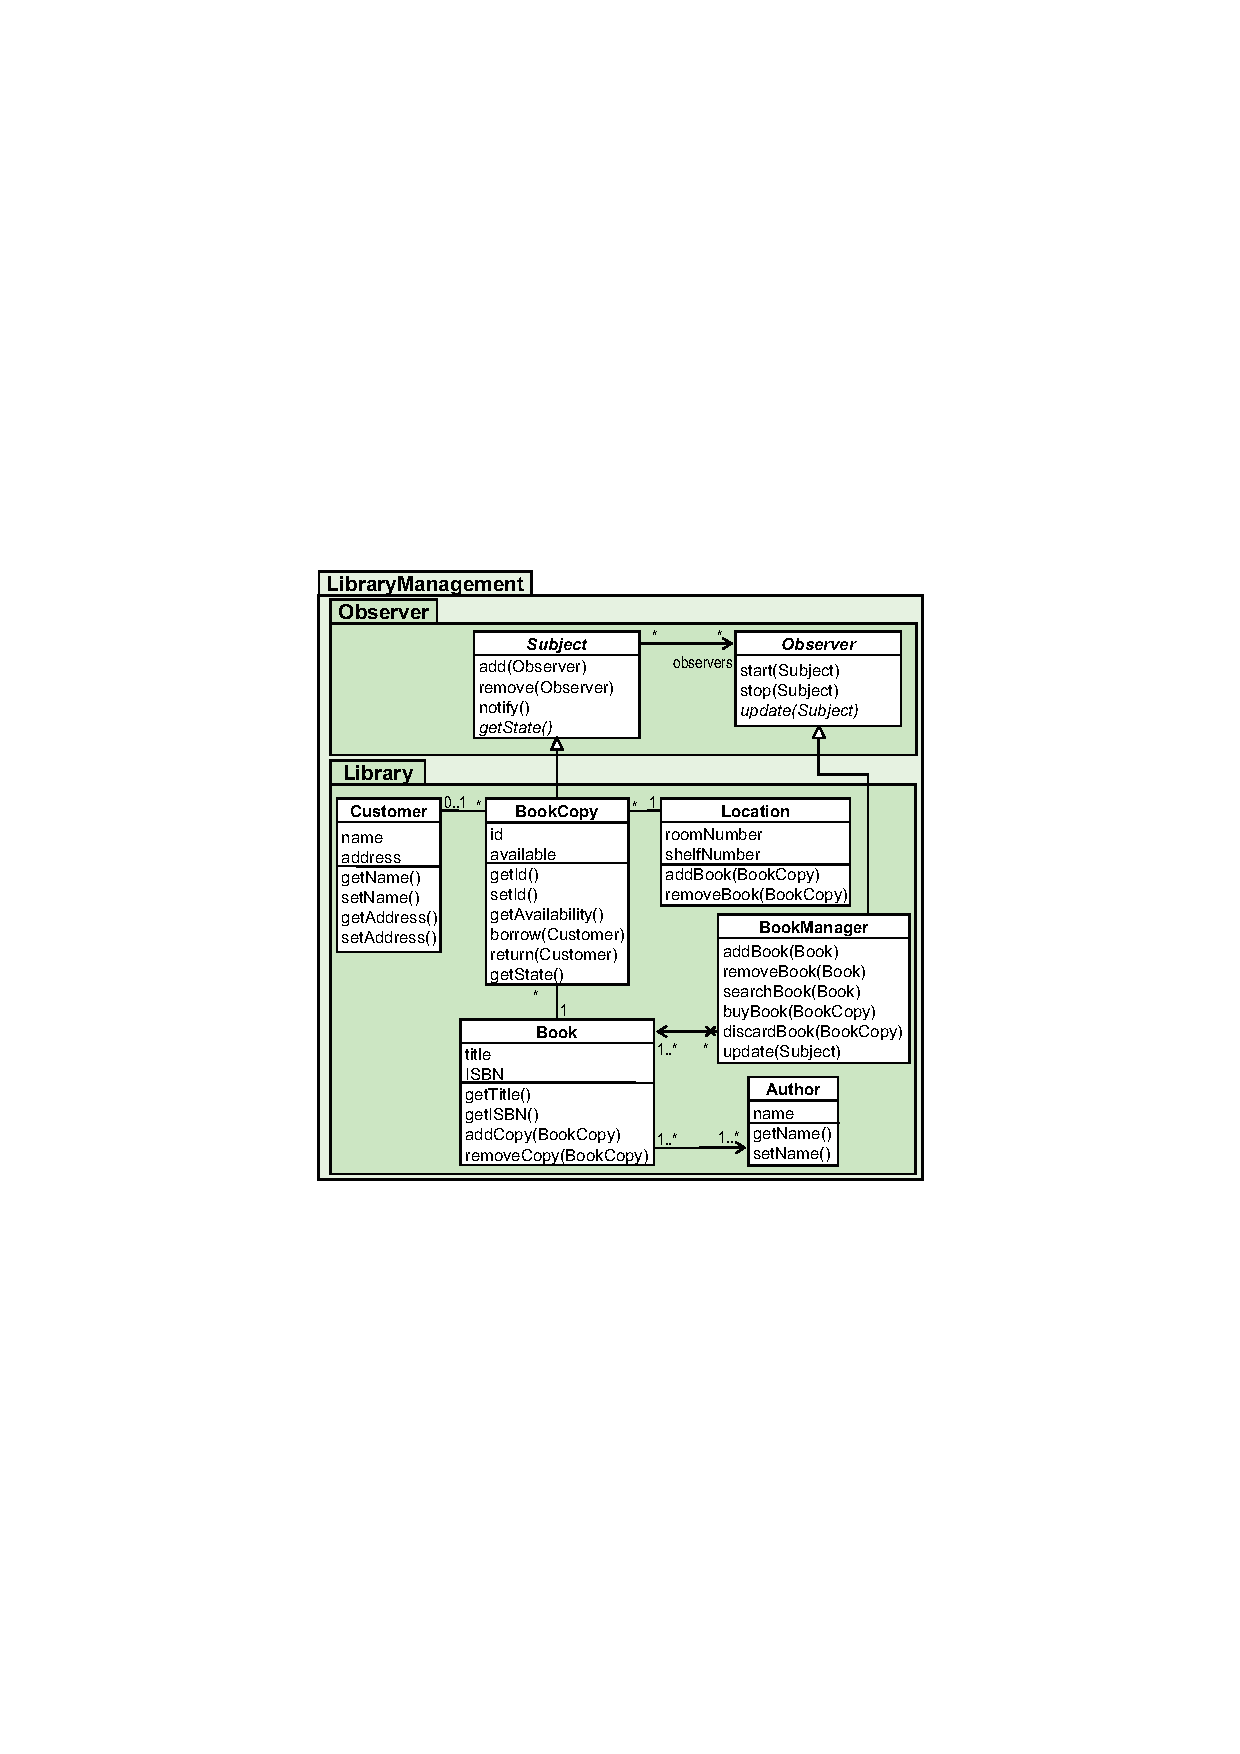
\includegraphics[width=0.4\linewidth]{figures/figure1}
	\caption{xxx (Quelle zitieren, wenn nicht selbst erstellt)}
	\label{fig:xxx}
\end{figure}
Tabellen
Jede Tabelle muss im Fließtext referenziertw werden. Für Tabellen gelten die selben Regeln, wie für Abbildungen (siehe dazu Abschnitt \ref{sec:abbildungen}).

Eine Beispiel einer Tabelle ist in Tabelle \ref{tab:xxx} zu finden:
\begin{table}
	\centering
	\begin{tabular}{| >{\bfseries}l | c | r | }
		\hline
			\rowcolor{orange} \bfseries Linksbündig & \bfseries Zentriert & \bfseries Rechtsbündig \\
		\hline
		\hline
			Zeile 1 & xxx & xxx \\\hline
			Zeile 2 & xxx & \dots \\\hline
			\multirow{2}{*}{Zeile3}
			& xxx & xxx \\\cline{2-3}
			& xxx & xxx \\\hline
		\hline
			\multicolumn{3}{| c |}{xxx} \\\hline
	\end{tabular}
	\caption{xxx (Quelle angeben)}
	\label{tab:xxx}
\end{table}

Bitte beachten Sie, dass Tabellen generell so einfach wie möglich gehalten werden sollen. Tabelle \ref{tab:xxx} dient unter anderem dazu Studierenden zu zeigen, wie Tabellen in \LaTeX\xspace erstellt werden können und wie Farben verwendet werden.